\subsection{Layers}
\label{sec:layers}

We start by analyzing layers in terms of size and compressibility, file and
directory counts, and layer directory depths.

\paragraph{Layer size and compressibility}

\begin{figure}[t]
	\centering
		\begin{minipage}{0.24\textwidth}
			\centering
			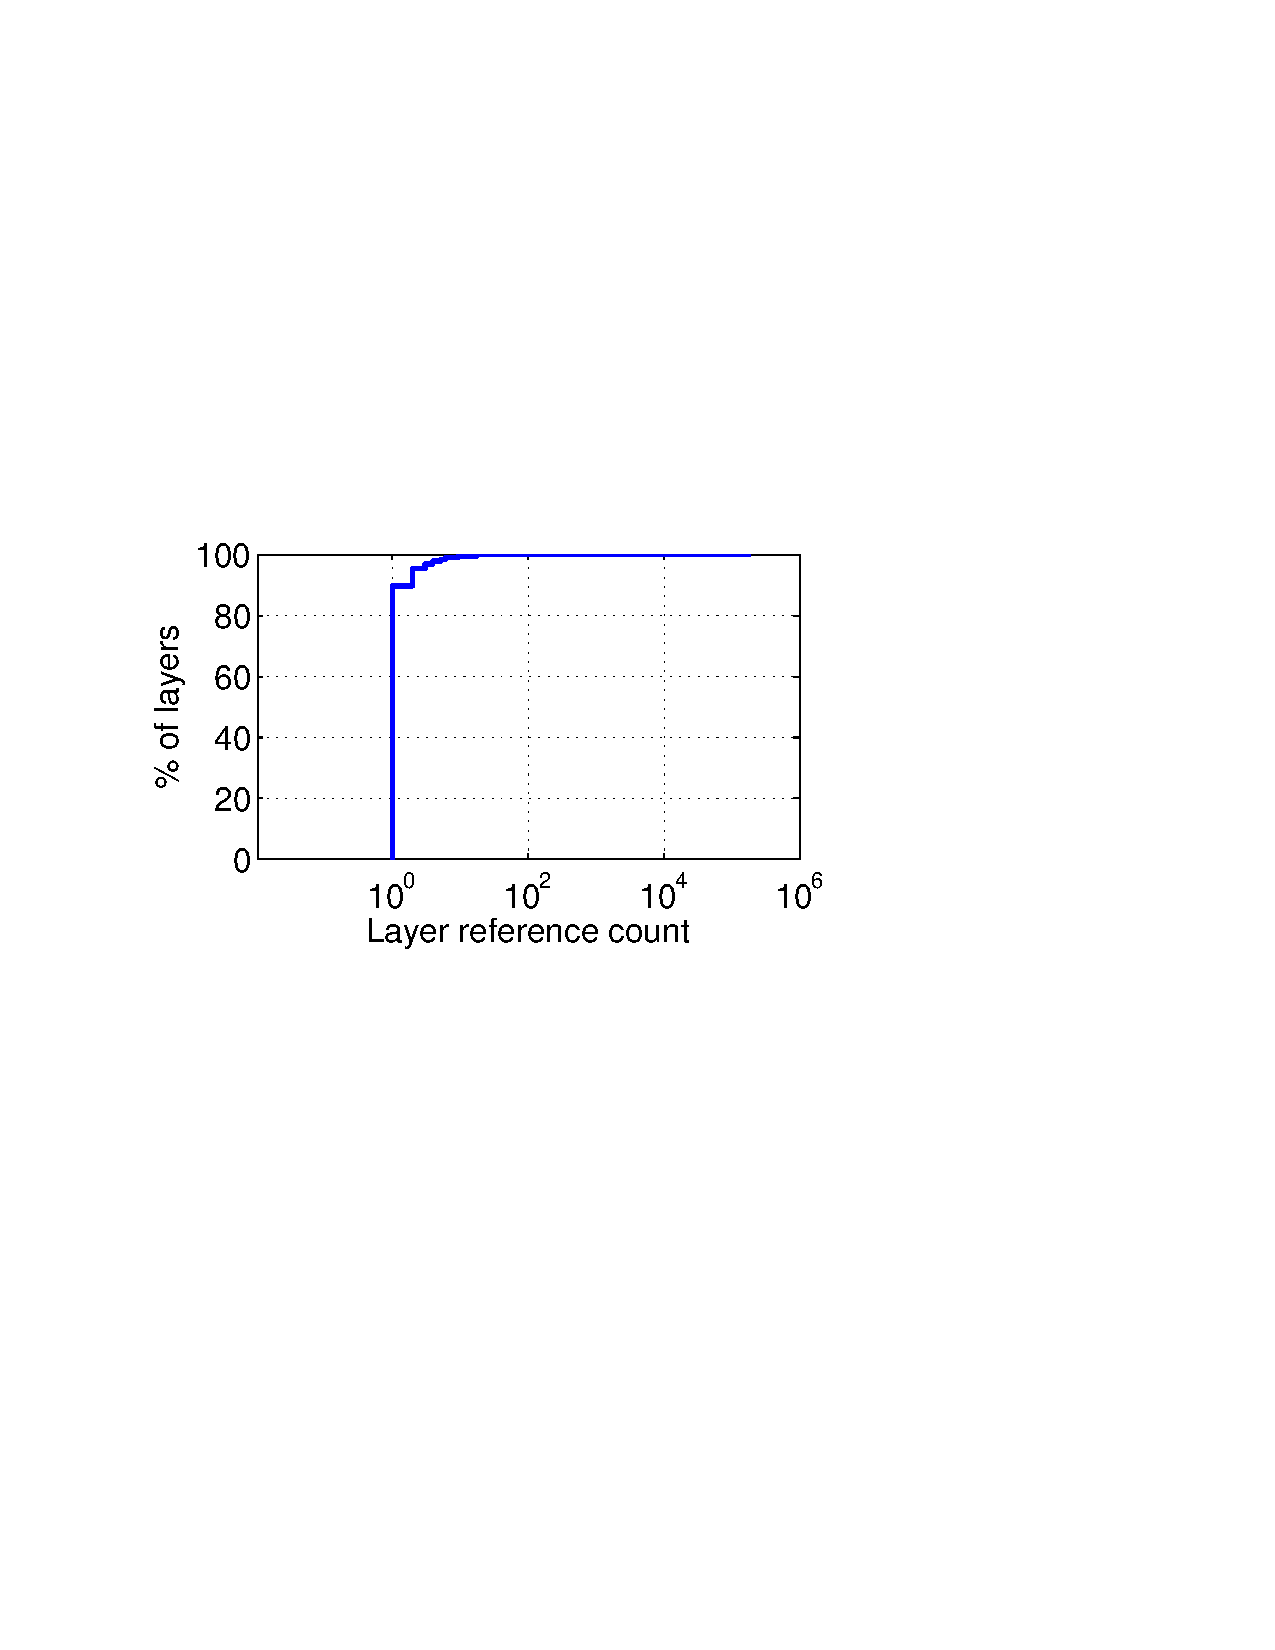
\includegraphics[width=1\textwidth]{graphs/shared-cnt-cdf.pdf}
			\caption{CDF of layer\\\ reference count.}
			\label{fig:ref_count}
		\end{minipage}
	\begin{minipage}{0.22\textwidth}
		\centering
		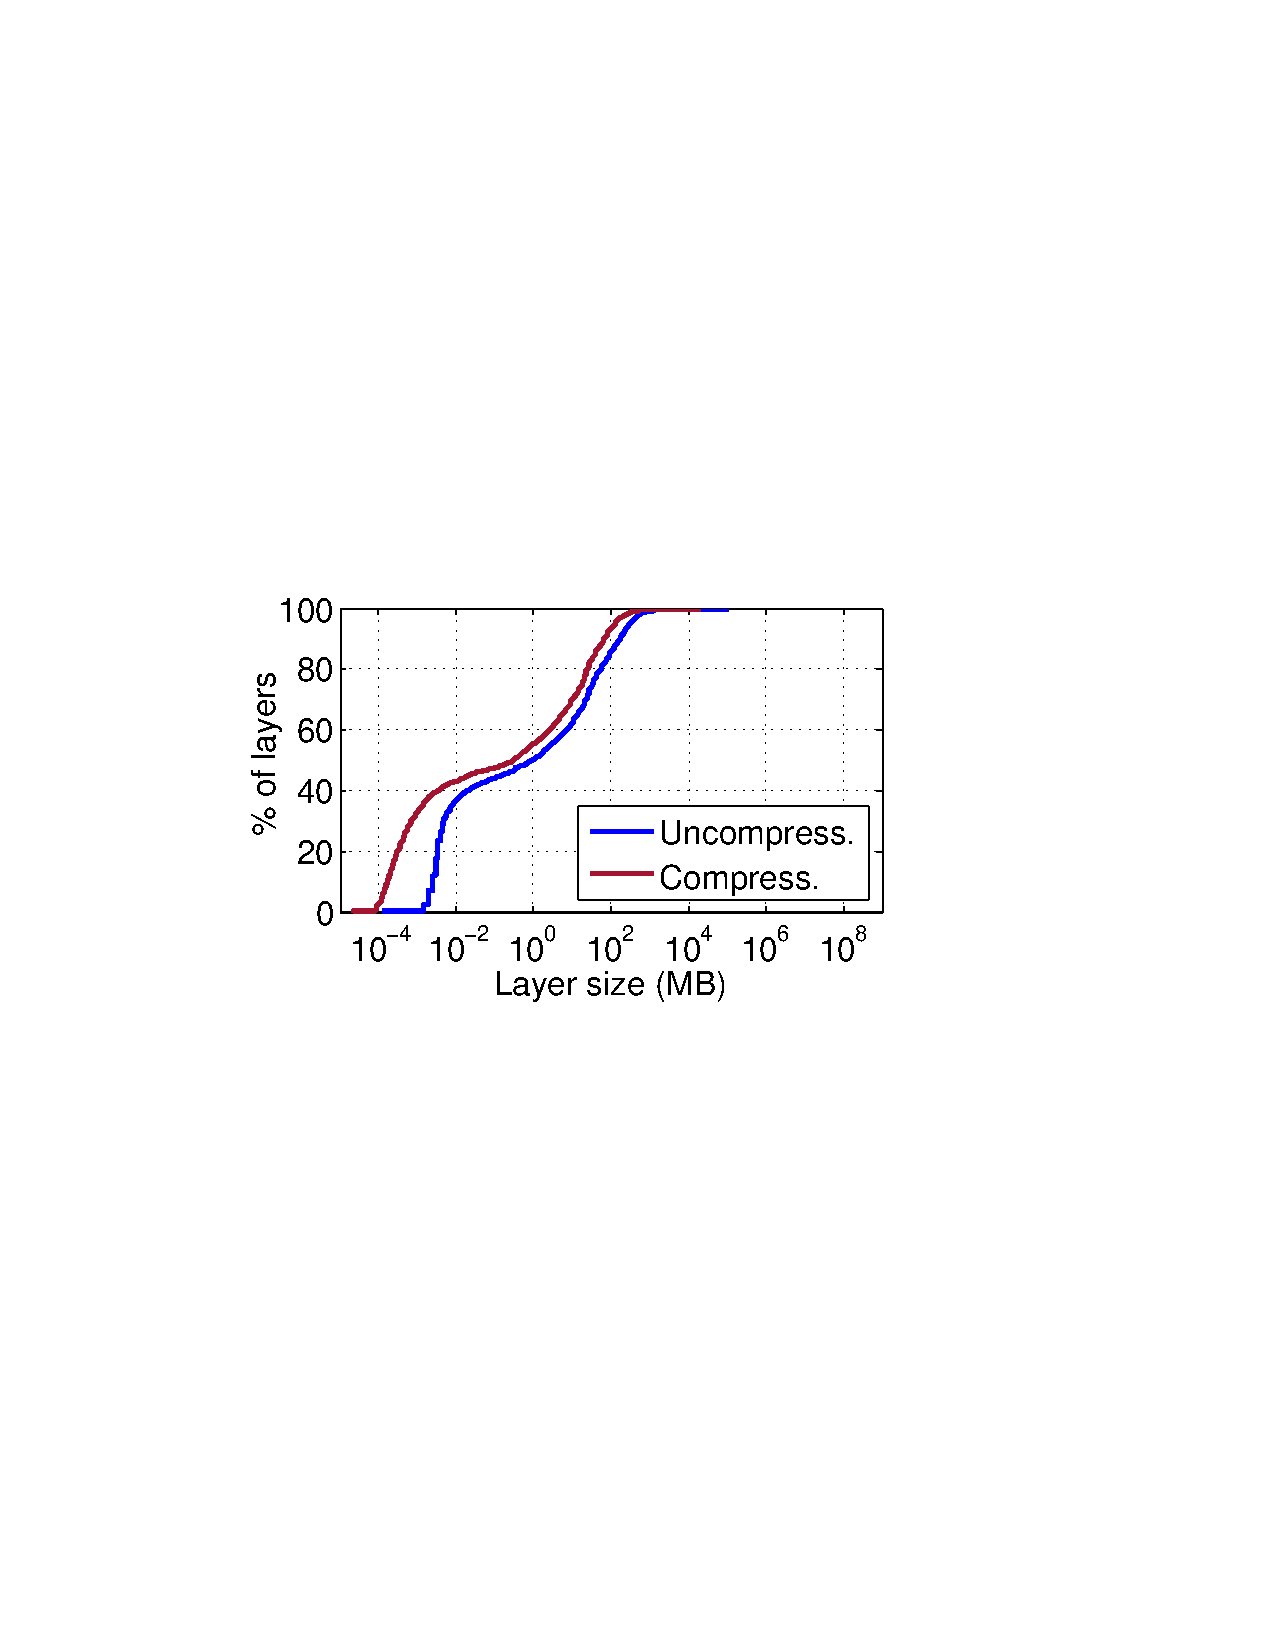
\includegraphics[width=1\textwidth]{graphs/layer-size-cdf.pdf}
		\caption{CDF of compress. and uncompress. layer size.}
		\label{fig:layer-size-cdf}
	\end{minipage}
\end{figure}


Figure~\ref{fig:layer-size-cdf} presents compressed and uncompressed layer size
distributions.
%
\vcomment{add a sentence explaining what compression algorithm and level is
used.}
%
We find that 50\% of the layers are less than 1MB and 90\% of the layers are
less than 64MB in compressed format.
%
\vcomment{Given that the corresponding graph uses 10 base on X axis, can we
replace 64MB above with 100MB and corresponding percentage (seems like around
95\%)}
%
If uncompressed, 50\% of the layers are smaller than 2 MB and 90\% of the
layers are smaller than 170MB.
%
\vcomment{Given that the corresponding graph uses 10 base on X axis, can we
replace 170MB above with 100MB and corresponding percentage (seems like around
85\%)}
%
\emph{Relatively small size of many layer allows to consider selective
in-memory layer caching at the registry side.}
%
We also calculated the layer compression ratio a shown in
Figure~\ref{fig:compress-ratio}.
%
We see that 80\% of the layers have compression ratio of \vcomment{XXX} or
higher and 50\% of layers have compression ratio larger than \vcomment{XXX}.
%
\emph{High compression ratio shows the potential of compression while
distributing the container images.}
%
\vcomment{Isn't it what Docker already does?}

% VASILY: I commented the text below out as 3\% seems to be a very
%  	  minor number.  Correct me if you think otherwise.
%-------------------------------------------------------------------
%However, looking at Figure~\ref{fig:compress-ratio},
%Figure~\ref{fig_hist_layer} we find that there are 3\% of layers for which the
%compression ratio is around 1.
%
%Doing compression and uncompression of such layers incur additional overhead at
%docker engine side.
%
%For such layers, we suggest not to do compression.
%
%Docker engine can use a hybrid approach to compress only those layers which
%yield better compression ratio.
%
%\emph{This way users pulling such layers do not need to uncompress and will
%experience reduction in container startup time.}
%-------------------------------------------------------------------

%\begin{figure}[!t]
%	\centering
%	\subfigure[CDF of layer depth]{\label{fig_reference_cnt_cdf}
%		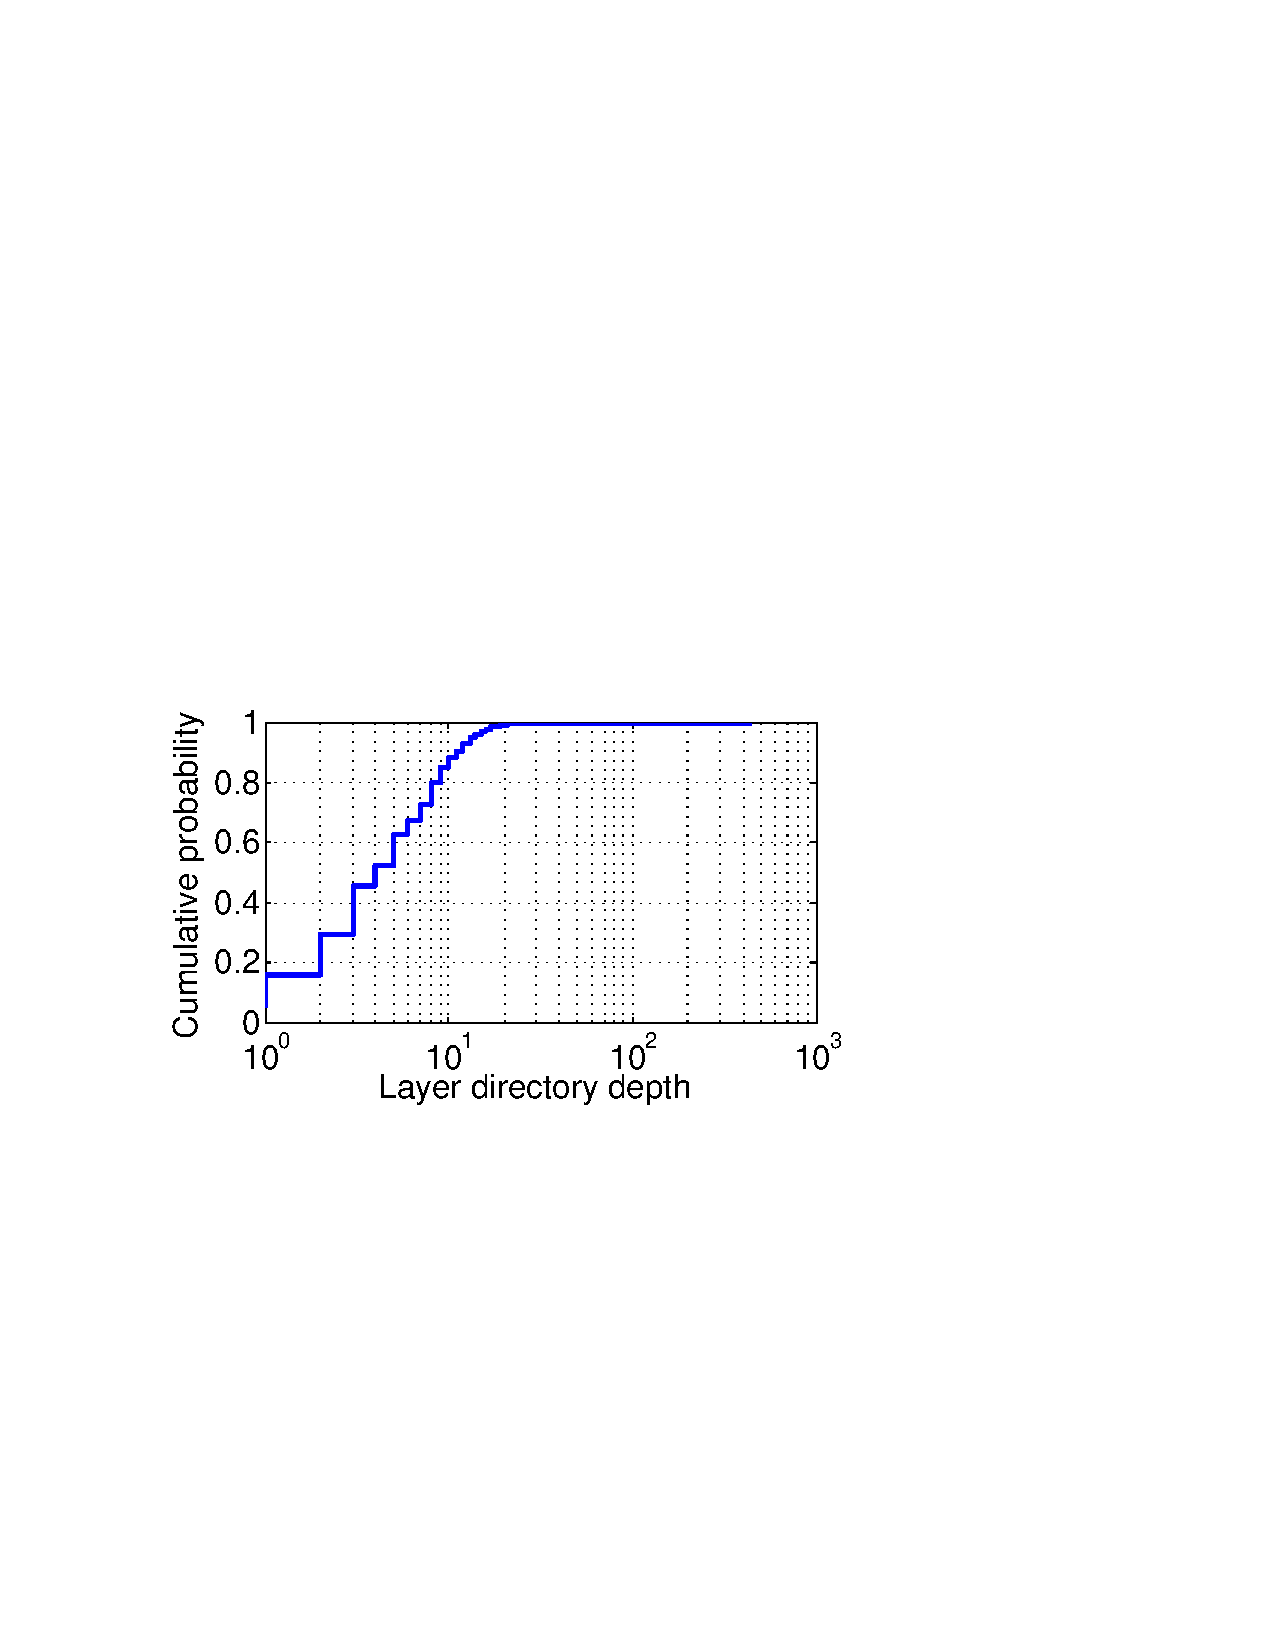
\includegraphics[width=0.21\textwidth]{graphs/layer-depth-cdf.pdf}%
%	}
%	\subfigure[Histogram of layer depth]{\label{fig_reference_cnt_pdf}
%		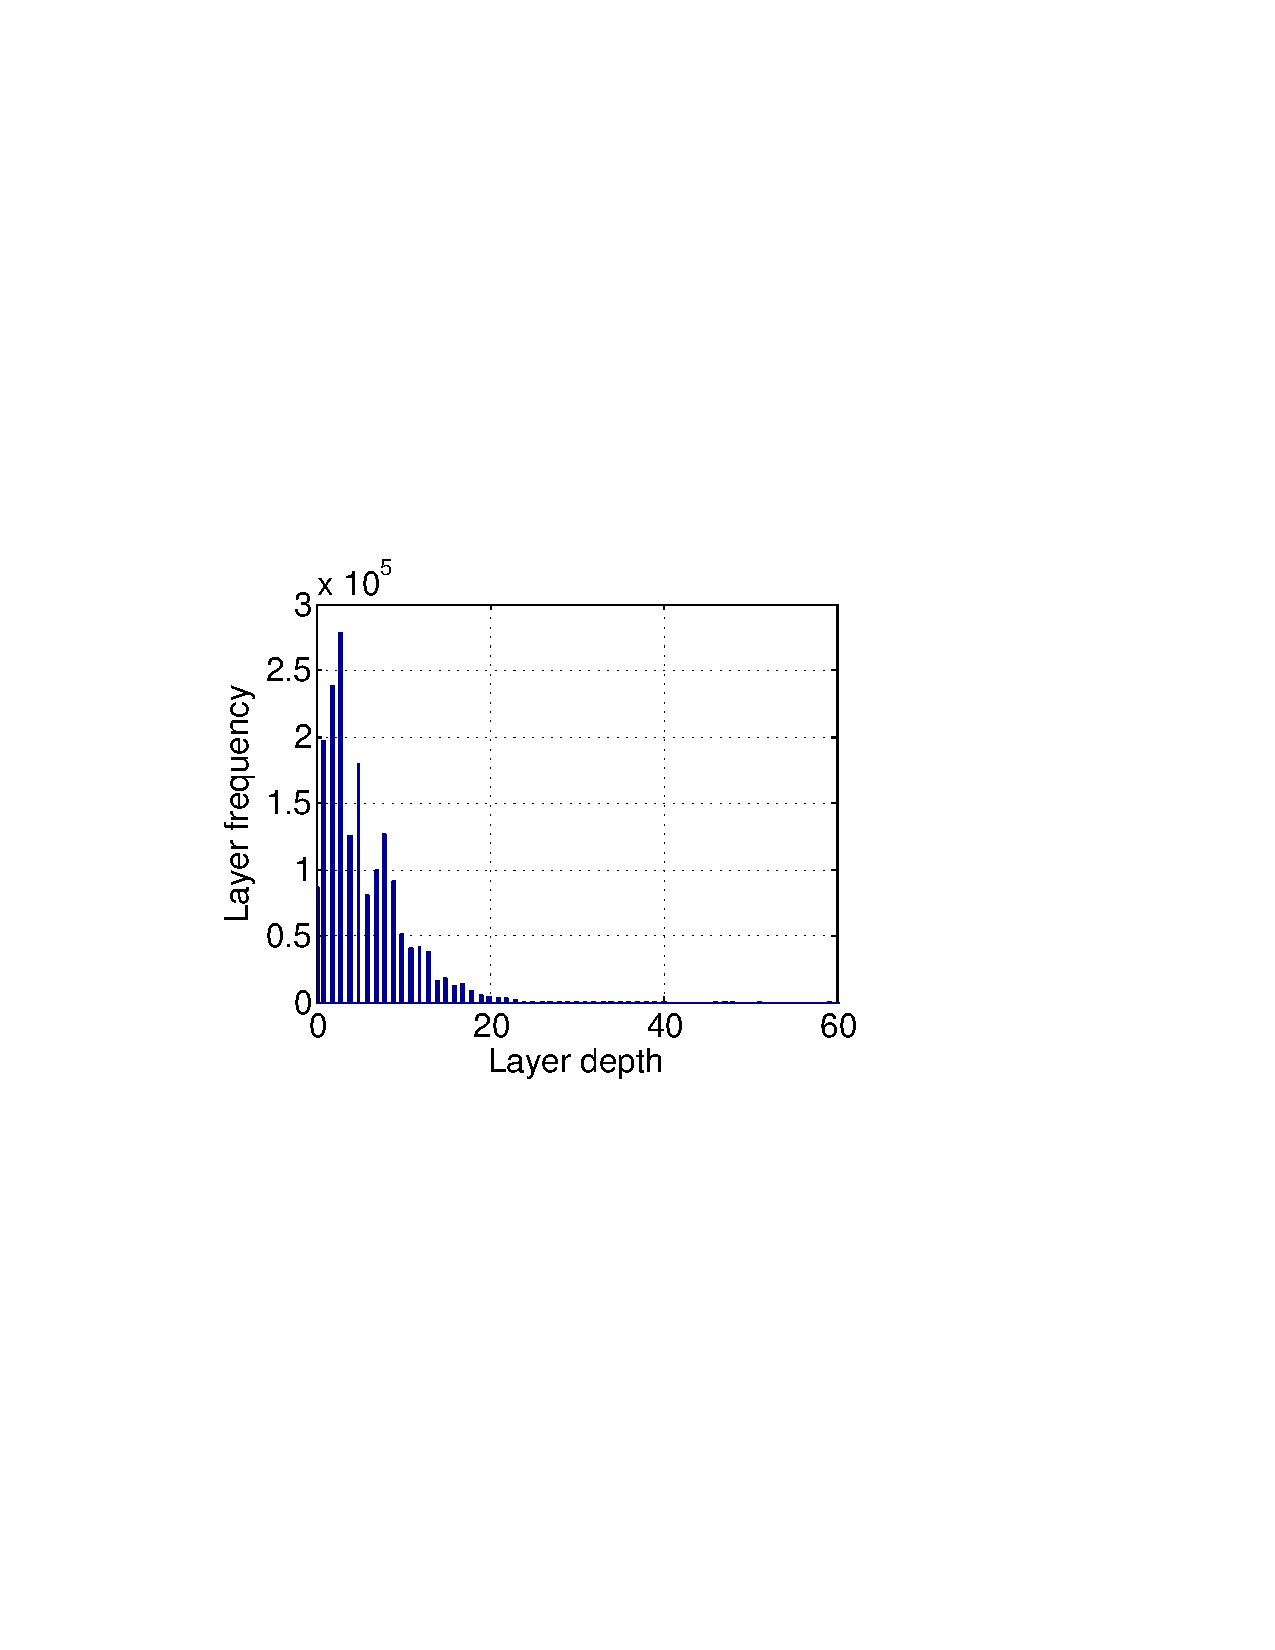
\includegraphics[width=0.21\textwidth]{graphs/layer-depth-pdf.pdf}
%	}
%	\caption{Layer depth distribution}
%	\label{fig:reference-cnt}
%\end{figure}

%Our size analysis reveals an interesting trade-off. Compression is
%computationally expensive and is one of the major sources of latency when
%pulling an image from Docker Hub~\cite{slacker}.  As the majority of layers is
%small and has low compression ratios, it can be beneficial to store small
%layers uncompressed in the registry to reduce pull latencies.


\paragraph{File and directory structure}

\begin{figure}[t]
	\centering
	\begin{minipage}{0.22\textwidth}
		\centering
		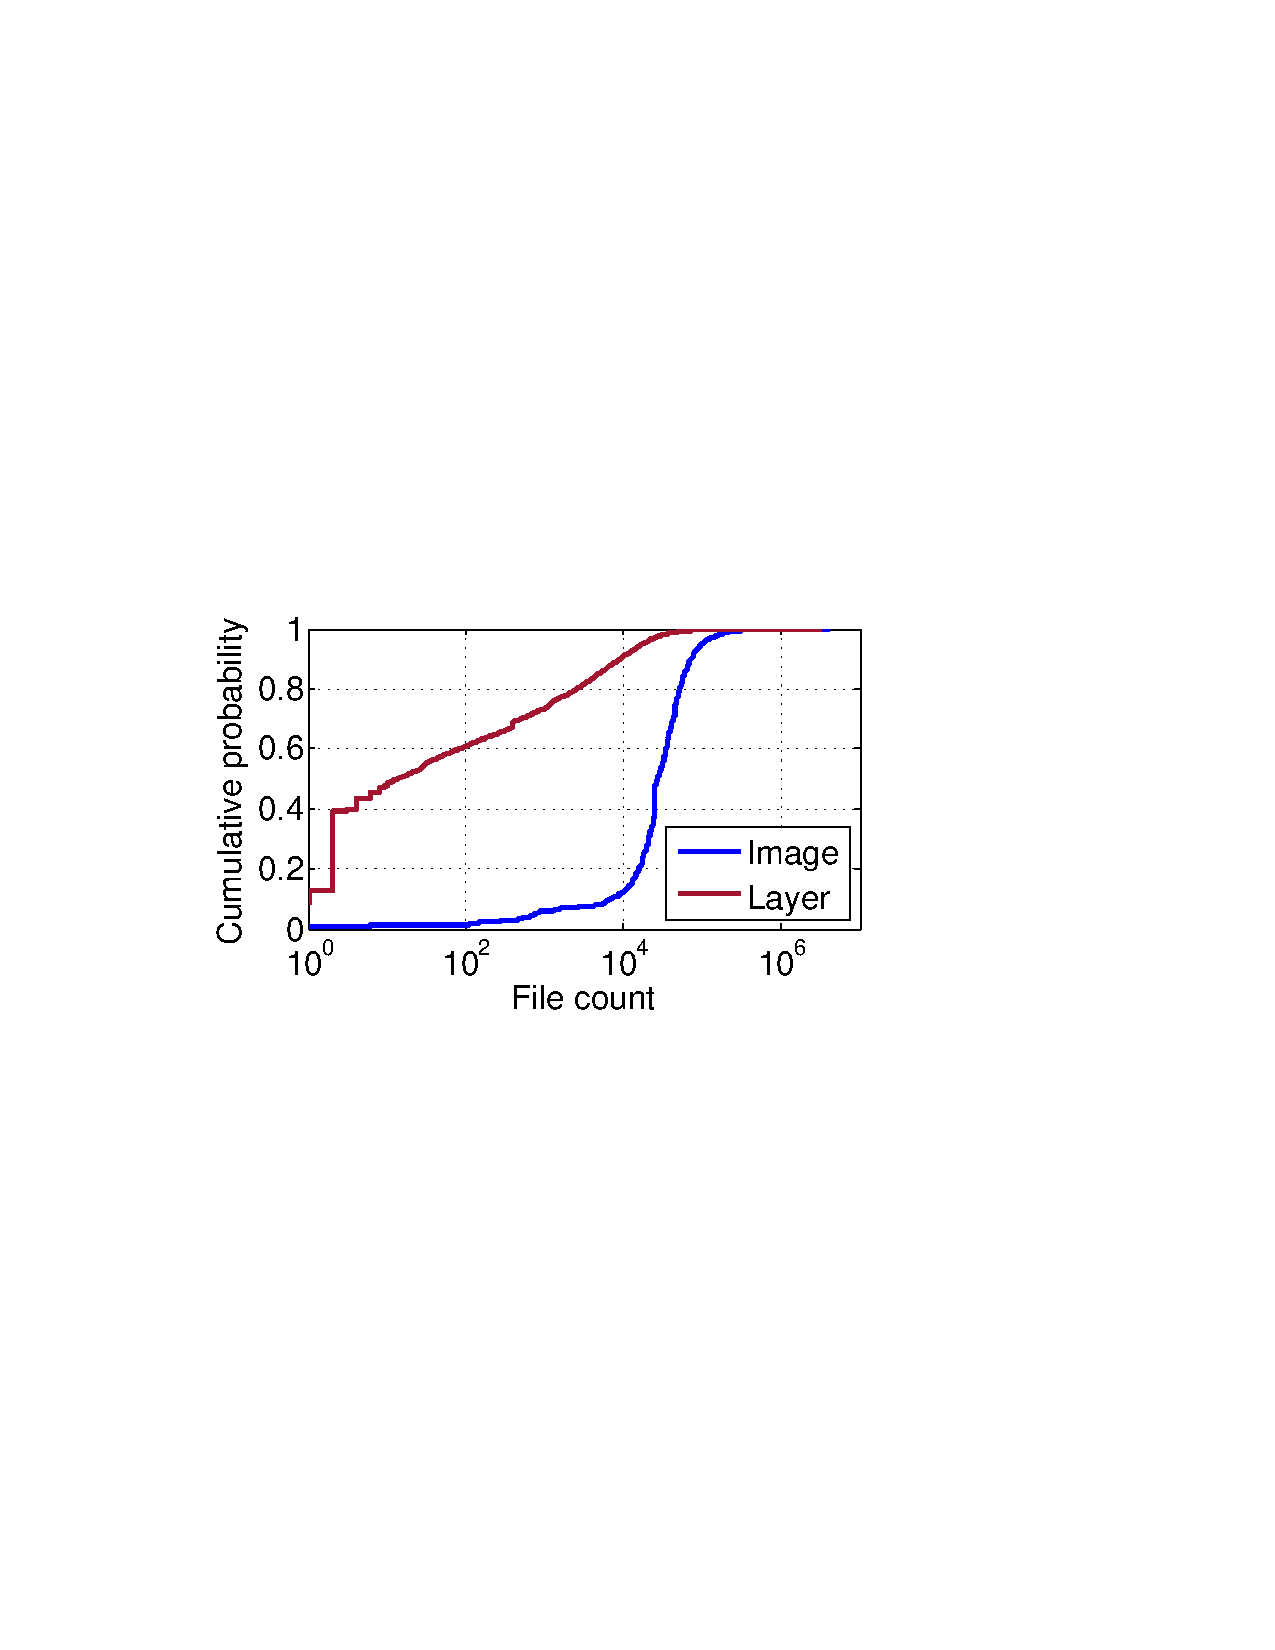
\includegraphics[width=1\textwidth]{graphs/file-cnt-cdf.pdf}
		\caption{CDF of file count.}
		\label{fig:file-cnt-cdf}
	\end{minipage}
	\begin{minipage}{0.22\textwidth}
		\centering
		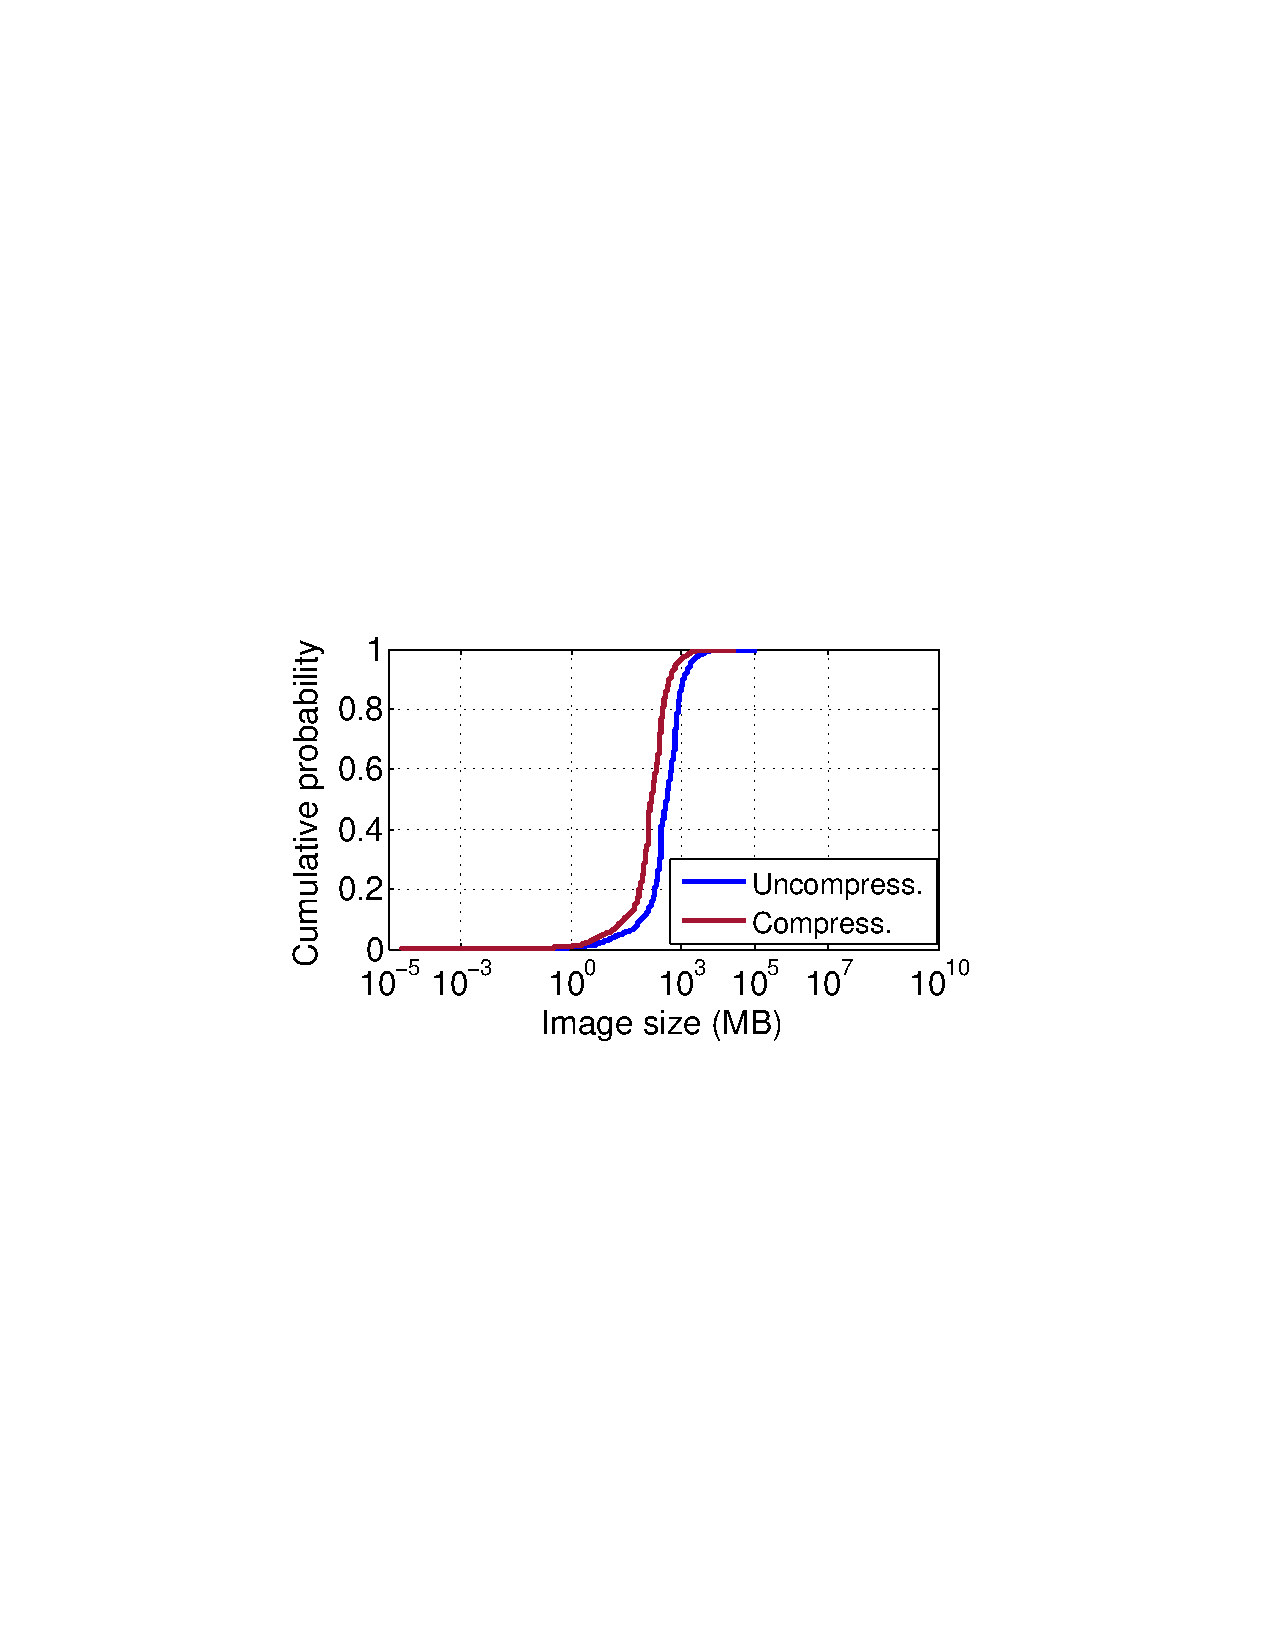
\includegraphics[width=1\textwidth]{graphs/image-size-cdf.pdf}
		\caption{CDF of image size (MB)}
		\label{fig:image-size-cdf}
	\end{minipage}%
\end{figure}

\begin{figure}[t]
	\centering
	\begin{minipage}{0.22\textwidth}
		\centering
		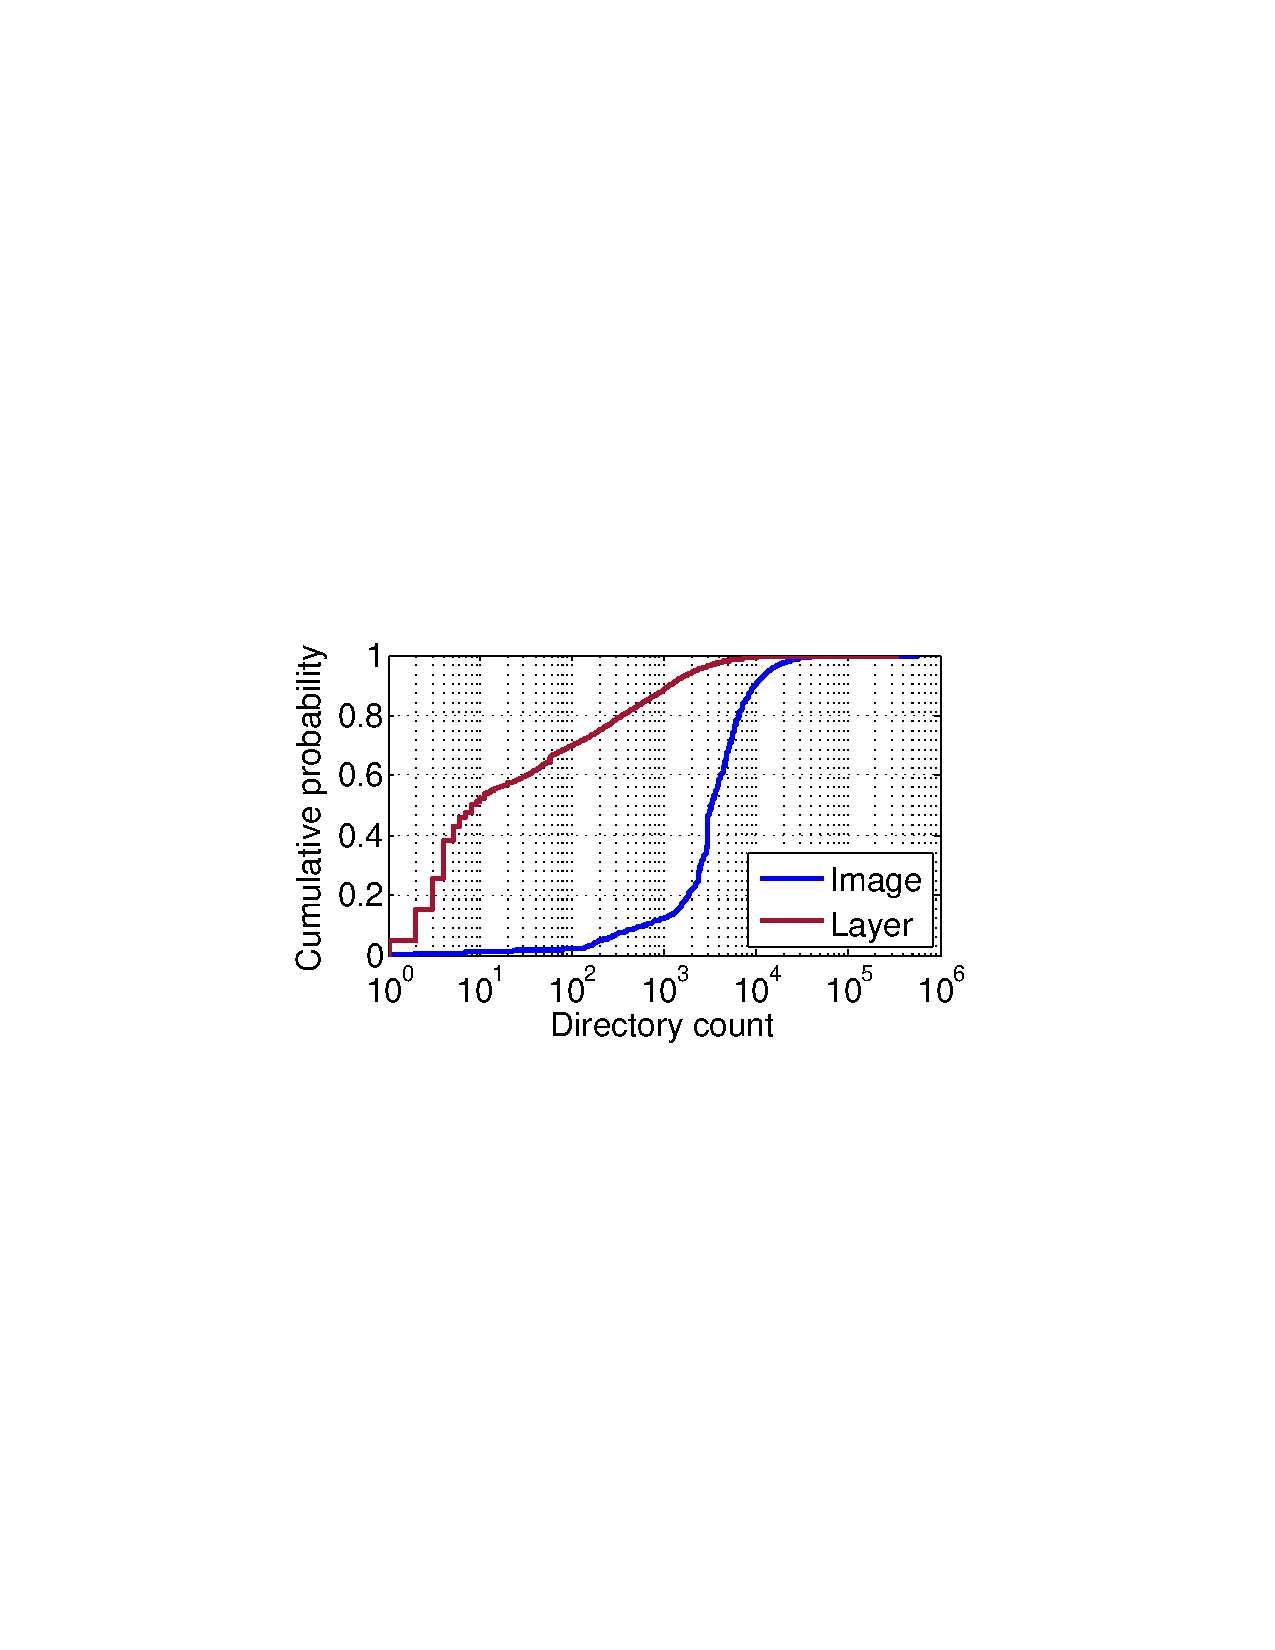
\includegraphics[width=1\textwidth]{graphs/dir-cnt-cdf.pdf}
		\caption{CDF of directory count}
		\label{fig:dir-cnt-cdf}
	\end{minipage}%
	\begin{minipage}{0.22\textwidth}
		\centering
		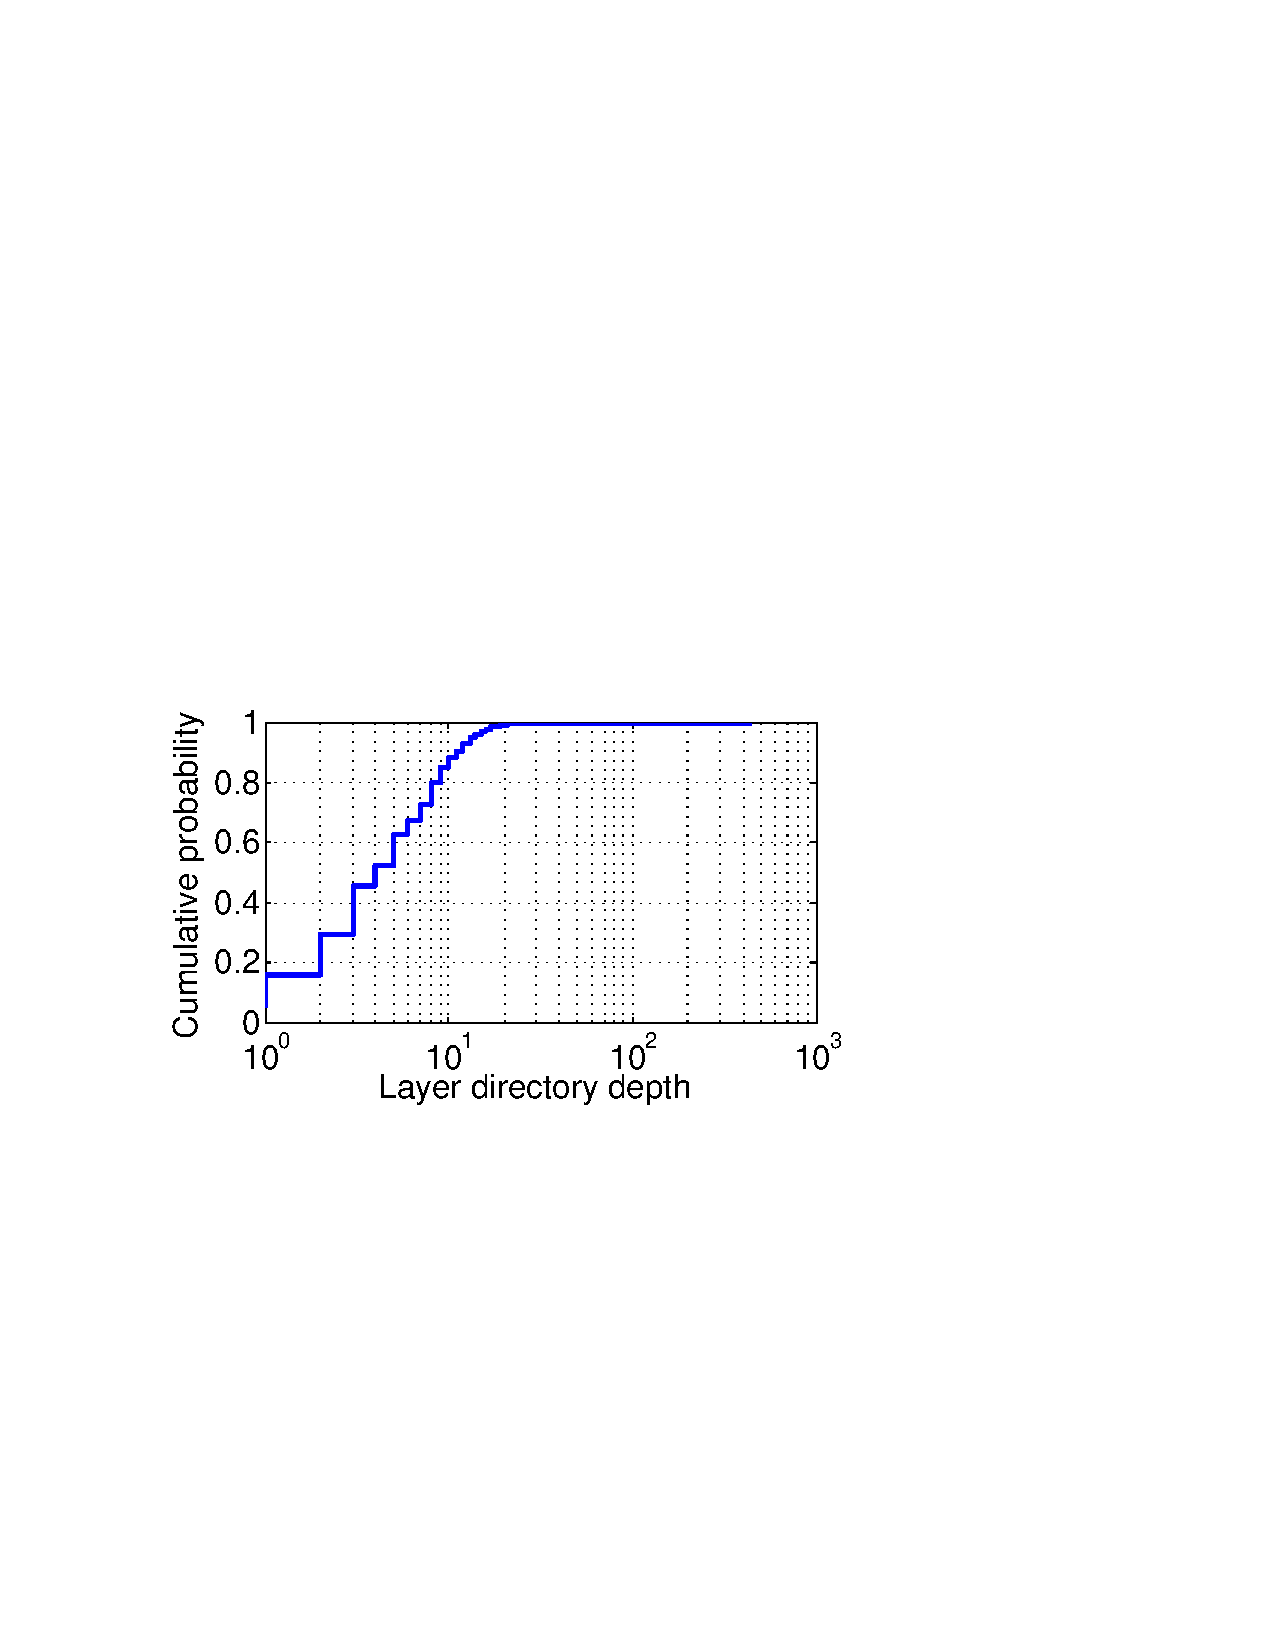
\includegraphics[width=1\textwidth]{graphs/layer-depth-cdf.pdf}
		\caption{CDF of layer directory depth}
		\label{fig:layer-depth-cdf}
	\end{minipage}
\end{figure}



We examine internal layer structure to determine if extracted
layers require large amounts of metadata from the storage system.
%
To further understand the metadata overhead, we decompressed the layer gzip
compressed archival file as a layer directory and counted the layer directory
depth as the maximum directory depth of its containing directories as shown in
%
Figure~\ref{fig:file-cnt-cdf} shows the CDF of the number of files per layer.
%
90\% of the layers contain less than 10,000 files while half of the layers have
less than 12 files.
%
Interestingly, 13\% of the layers have only a single file.
%
\vcomment{here we need to give some hint what are those files?}
%
Figure~\ref{fig:dir-cnt-cdf} shows taht 70\% of layers have less than 100
directories and around 10\% of layers have more than 1,000 directories while
the median is 8.
%
Directory depth is shallow (\ref{fig:layer-depth-cdf}) as 50\% of layers have
less 4 levels in layer directory depth and 90\% of layers have less than 11
levels.
%
\emph{This analysis shows that the majority of layers consists only of a small
number of files an directories and does not contain deeply nested directory
hierarchies.
%
Hence, except a few outliers, unpacked layers do not require a large amount of
metadata from the storage system.}

%\nancomment{still metadata overhead}
%\begin{figure}
%	\centering
%	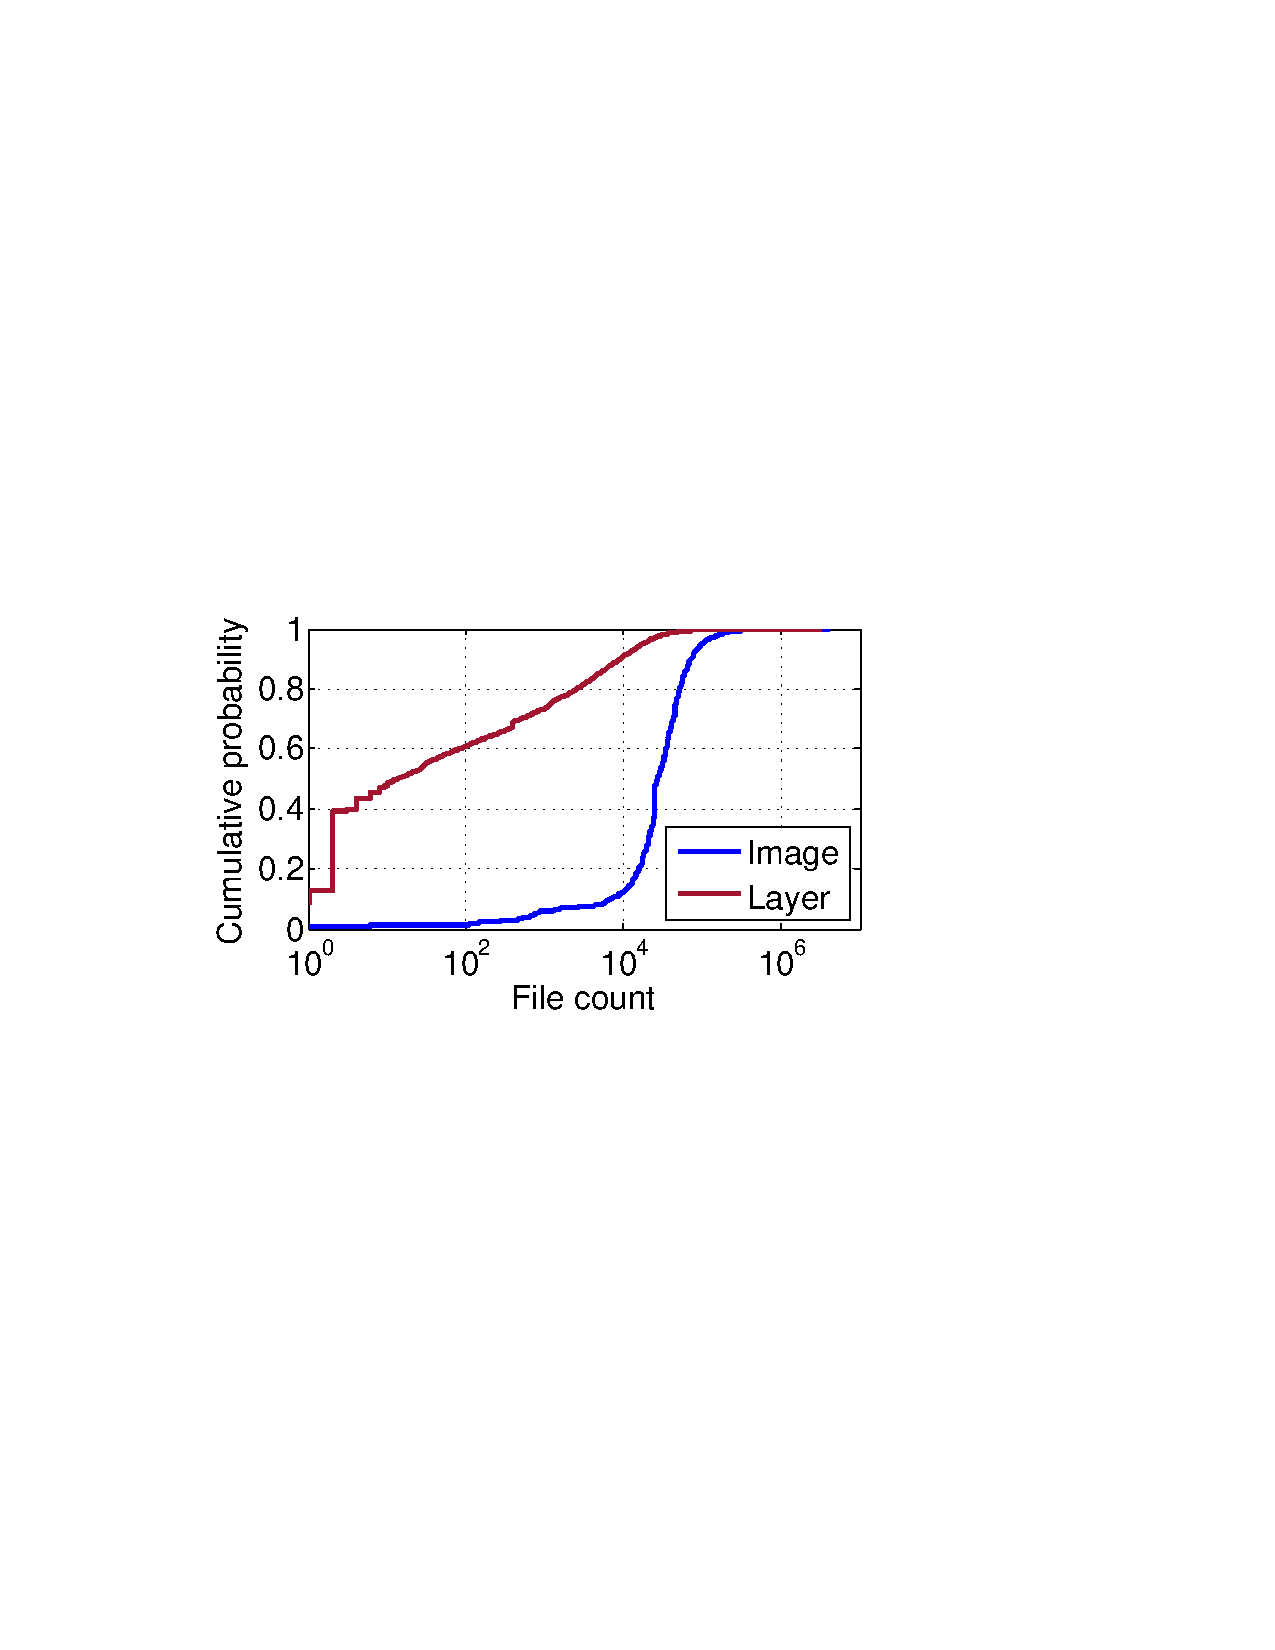
\includegraphics[width=0.4\textwidth]{graphs/file-cnt-cdf.pdf}
%	\caption{CDF of file count per image/layer.
%	}
%	\label{fig:reference-cnt}
%\end{figure}

%\begin{figure}[!t]
%	\centering
%	\subfigure[Histogram of directory count per image]{\label{fig_reference_cnt_cdf}
%		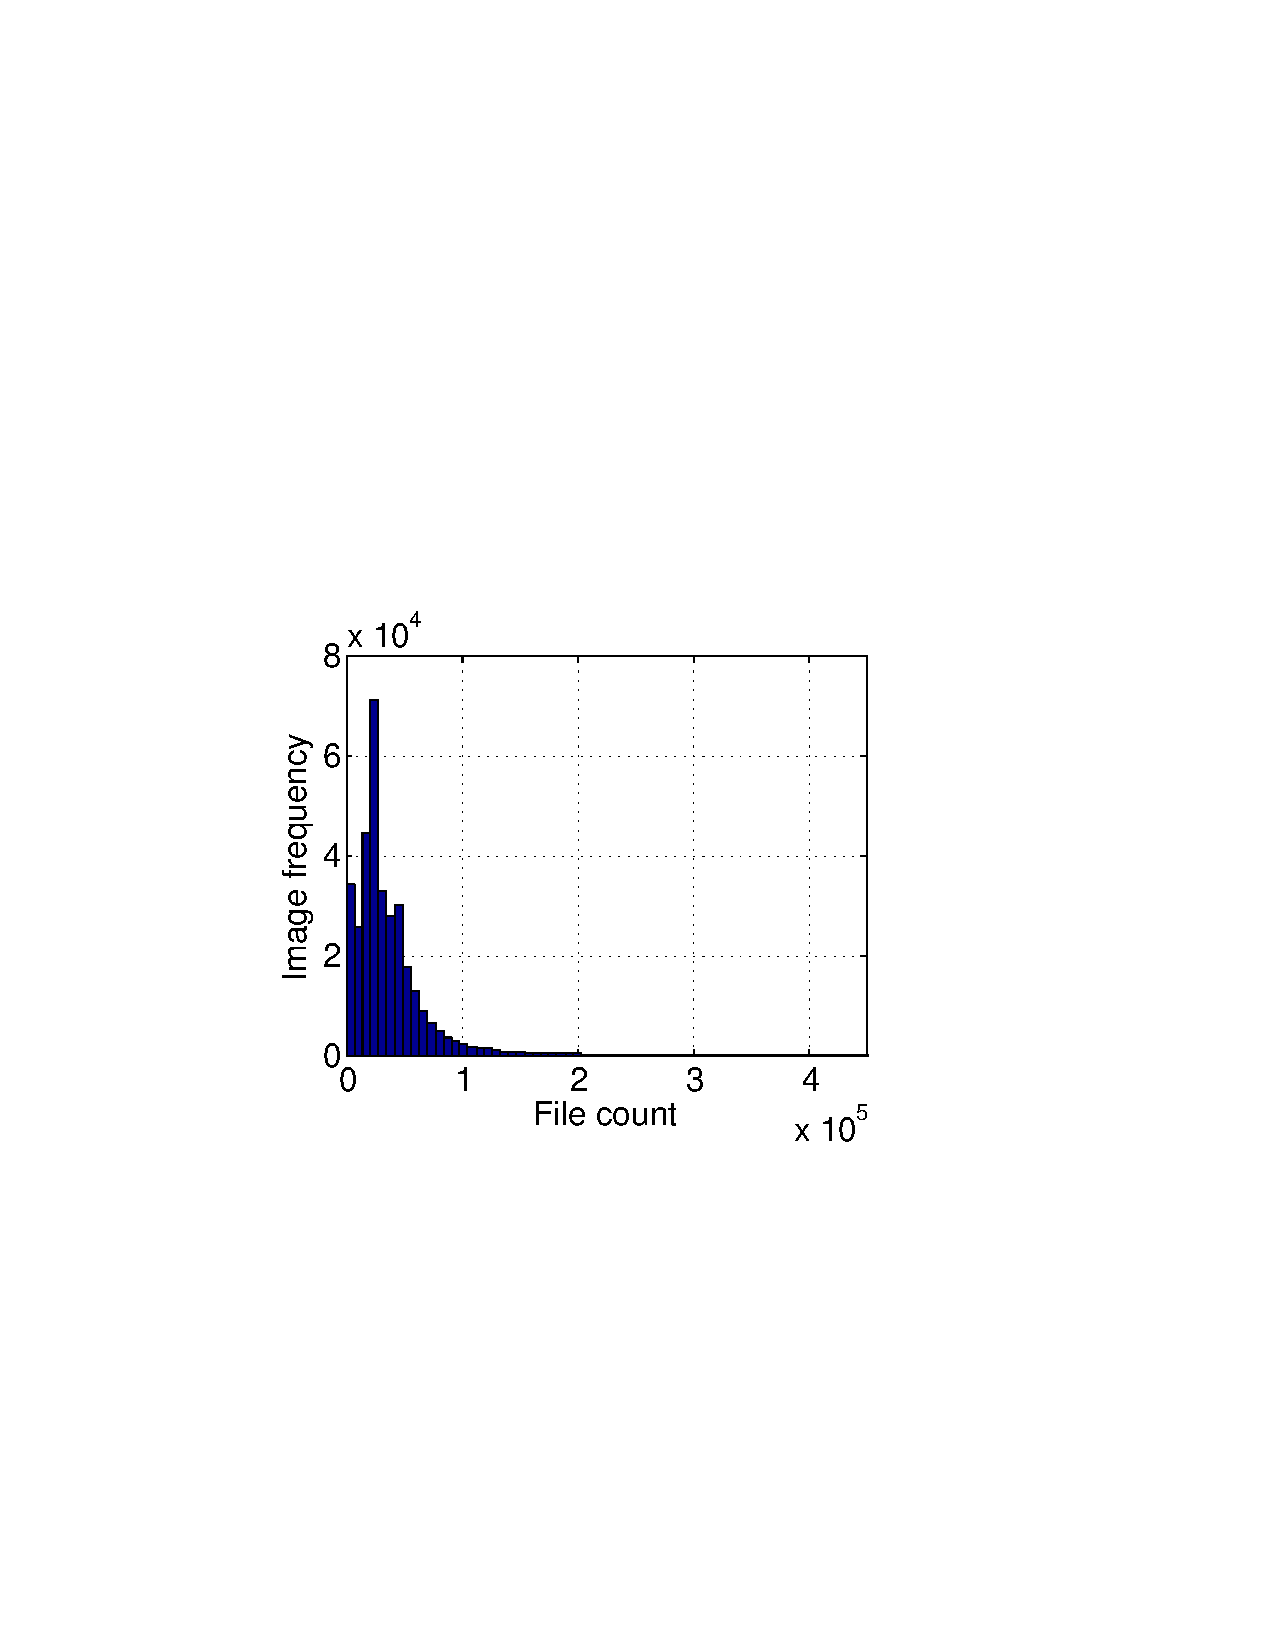
\includegraphics[width=0.21\textwidth]{graphs/image-file-cnt-pdf.pdf}%
%	}
%	\subfigure[Histogram of directory count per layer]{\label{fig_reference_cnt_pdf}
%		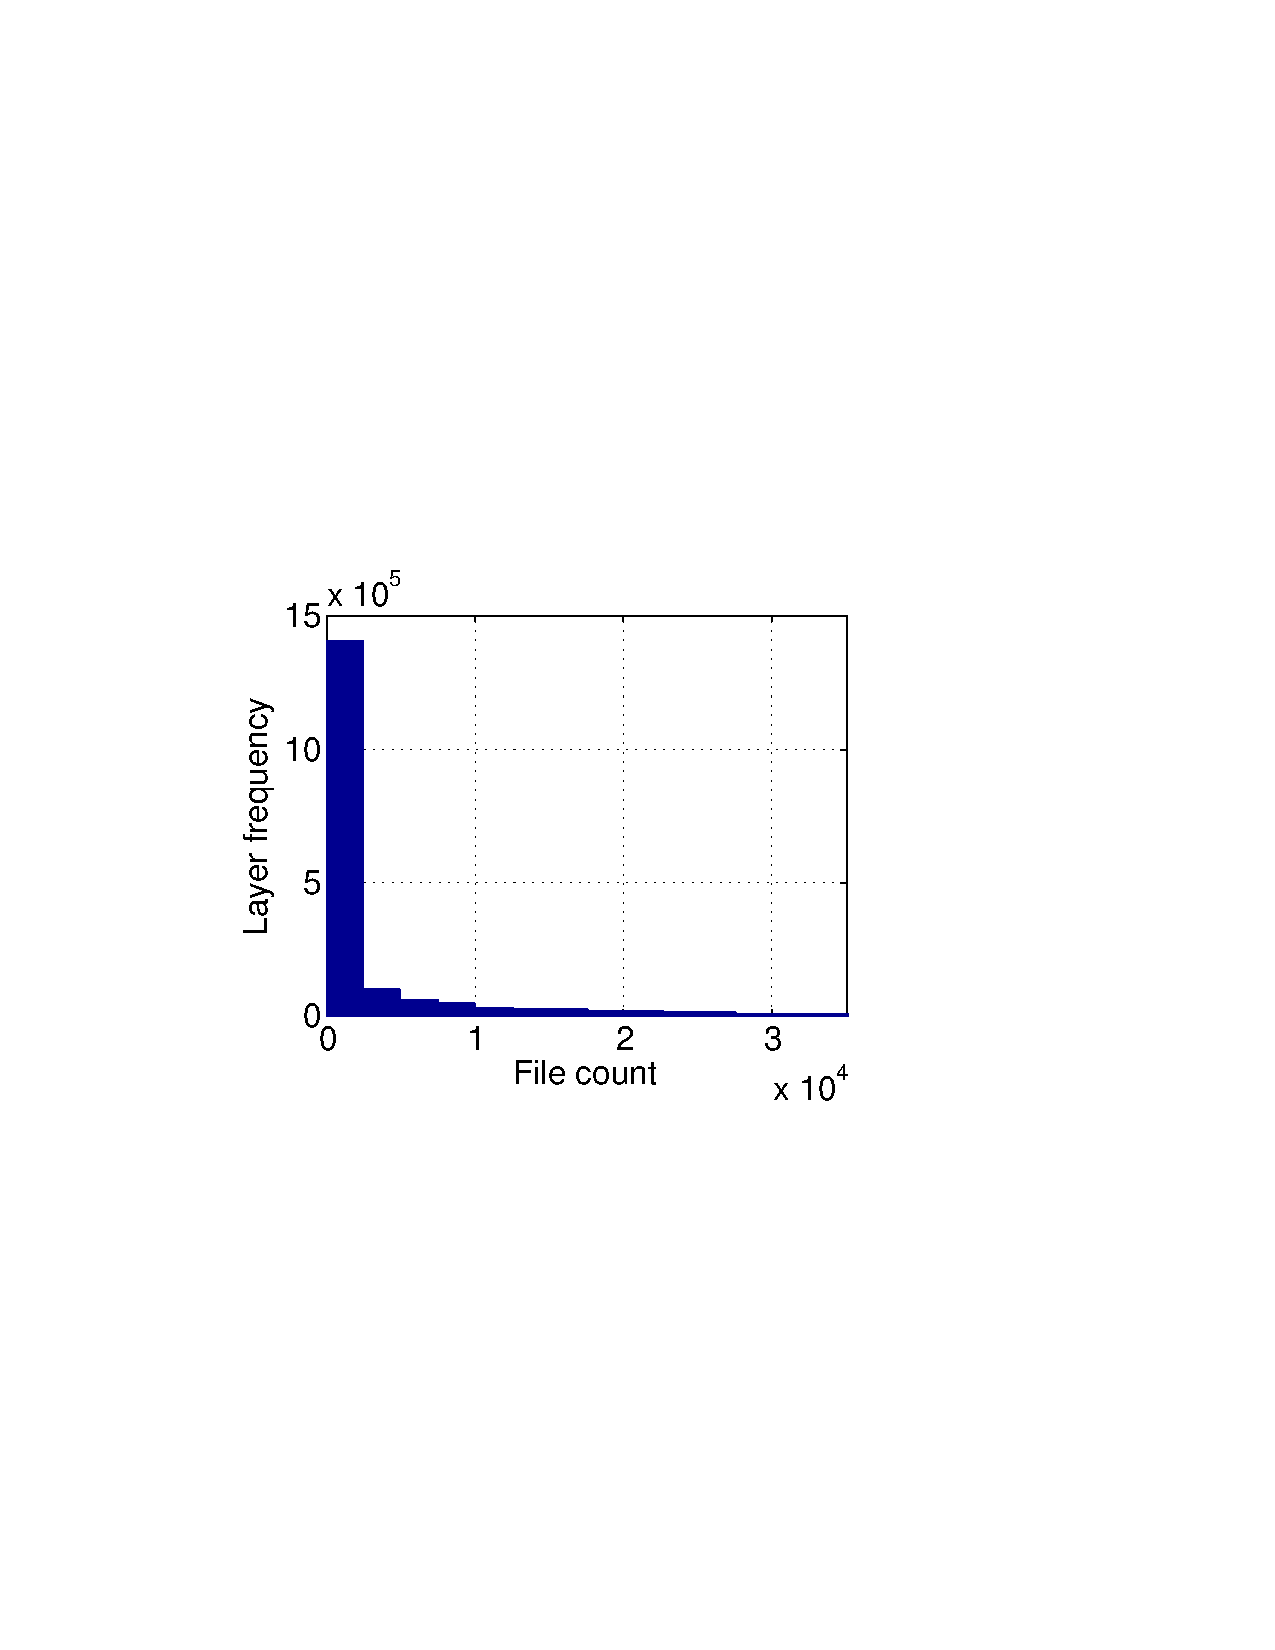
\includegraphics[width=0.22\textwidth]{graphs/layer-file-cnt-pdf.pdf}
%	}
%	\caption{Histogram of directory count distribution}
%	\label{fig:reference-cnt}
%\end{figure}


% while 7\% even
%showed no files at all. We currently do not know the exact reason for the
%layers without files, but one theory is that these layers use Docker volumes to
%store all requred files (including executables).
% plan to investigate their corresponding images in the future.
%\nancomment{The layers are not empty since it could have directories}.
%On the other hand, the largest layer contains 826,196 files and was part of a
%Debian image.
%
%The average is 2,200.
%
%For directories, 90\% of the layers have less than 826 directories and half of
%the layers consist of less than 11 directories. We again observe a wide range
%with a minimum of a single directory and a maximum of 111,940. The layer with
%the most directories was part of the \emph{conjurinc/developer-quiz} image.

%\paragraph{Directory depths}

%After extracting and unpacking gzip compressed layer archival files,
%Besides the count, we also calculate the maximum directory depth for each layer
%(Figure~\ref{fig_layer_depth}).
%%
%Around 90\% of all layers have a directory depth less than 10 while for 50\% of
%the layers, the directory depth is less than 4.
%
%The most frequent directory depth is 3 with 313,000 layers showing this depth
%value (Figure~\ref{fig_hist_layer_depth}).
%
%About 313,000 layers' layer directory depth is 3, which is the peak value in
%the figure.
%
%The maximum repeat count is 444 while the median is 4. The average is ~5.
